\documentclass[
% -- opções da classe memoir --
    12pt,       % tamanho da fonte
    %openright, % capítulos começam em página ímpar
    %twoside,   % frente e verso
    oneside,    % apenas um lado
    a4paper,    % tamanho do papel.
%
% -- opções da classe abntex2 --
    chapter=TITLE,	  	  % títulos de capítulos em letras maiúsculas
    %section=TITLE,		  % títulos de seções em letras maiúsculas
    %subsection=TITLE,	  % títulos de subseções em letras maiúsculas
    %subsubsection=TITLE, % títulos de sub-subseções em letras maiúsculas
%
% -- opções do pacote babel --
    english,			  % idioma adicional para hifenização
    % french,			  % idioma adicional para hifenização
    % spanish,            % idioma adicional para hifenização
    brazil				  % o último idioma é o principal do documento
%
]{abntex2}

\usepackage{mystyle}
\newcommand{\productname}{Hermes}

% -----------------------------------------------------------------------------
% Informações de dados para CAPA e FOLHA DE ROSTO
% -----------------------------------------------------------------------------
% \title{\productname: Uma prótese robótica para geração de ações em movimentos baseada em \textcolor{red}{padrões musculares \textbf{[trocar]}}}
\title{Automail-$X$: Prótese Robótica Autônoma para a Previsão de Movimentos de Caminhada baseada em Padrões Musculares}
\titulo{\thetitle}

\author{RODRIGO DOS SANTOS TAVARES}
\autor{\theauthor}

\local{Boa Vista --- RR}

\date{2018}
\data{\thedate}
\orientador{Dr.\ Herbert Oliveira Rocha}

\tipotrabalho{Monografia}

\preambulo{Monografia de Graduação apresentada ao Departamento de Ciência da
  Computação da Universidade Federal de Roraima como requisito parcial para a
  obtenção do grau de Bacharel em Ciência da Computação.}

% -----------------------------------------------------------------------------


% -----------------------------------------------------------------------------
% Informações de dado para a FOLHA DE APROVAÇÃO
% -----------------------------------------------------------------------------
%\renewcommand{\dataDefesa}{?? de ????? de 2017}%TODO:Data de defesa
\renewcommand{\orientadorBanca}{Prof.\ Dr.\ Herbert Oliveira Rocha}
\renewcommand{\primeiroMembroBanca}{Prof.\ Dr.\ Leandro Nelinho Balico}%TODO:Membros da banca
\renewcommand{\segundoMembroBanca}{Prof.\ Dr.\ Luciano Ferreira Silva}
% -----------------------------------------------------------------------------


% -----------------------------------------------------------------------------
% compila o índice
% -----------------------------------------------------------------------------
\makeindex
% -----------------------------------------------------------------------------

% -----------------------------------------------------------------------------
% Início do documento
% -----------------------------------------------------------------------------
\begin{document}

% Retira espaço extra obsoleto entre as frases.
%\frenchspacing

% -----------------------------------------------------------------------------
% ELEMENTOS PRÉ-TEXTUAIS
% -----------------------------------------------------------------------------
% \pretextual

% -----------------------------------------------------------------------------
% Capa
% -----------------------------------------------------------------------------
\imprimircapa{}
% -----------------------------------------------------------------------------

% -----------------------------------------------------------------------------
% Folha de rosto
% (o * indica que haverá a ficha bibliográfica)
% -----------------------------------------------------------------------------
\imprimirfolhaderosto{}
% -----------------------------------------------------------------------------

% -----------------------------------------------------------------------------
% Inserir folha de aprovação
% -----------------------------------------------------------------------------
\imprimirfolhadeaprovacao{}
% -----------------------------------------------------------------------------

% -----------------------------------------------------------------------------
% Dedicatória
% -----------------------------------------------------------------------------
% \begin{dedicatoria}
%   \vspace*{\fill}
%   \centering
%   \noindent
%   \textit{Dedicatória} \vspace*{\fill}%TODO: Dedicatória
% \end{dedicatoria}
% -----------------------------------------------------------------------------

% -----------------------------------------------------------------------------
% Agradecimentos
% -----------------------------------------------------------------------------
% \begin{agradecimentos}[Agradecimentos]
%   \textcolor{red}{\lipsum[1]}%TODO:Agradecimentos
% \end{agradecimentos}
% -----------------------------------------------------------------------------

% -----------------------------------------------------------------------------
% Epígrafe
% -----------------------------------------------------------------------------
% \begin{epigrafe}
%     \vspace*{\fill}
% 	\begin{flushright}
% 		\textit{???????????} %TODO: Epígrafe
% 	\end{flushright}
% \end{epigrafe}
% -----------------------------------------------------------------------------

% -----------------------------------------------------------------------------
% RESUMOS
% -----------------------------------------------------------------------------
\setlength{\absparsep}{18pt} % ajusta o espaçamento dos parágrafos do resumo

% -----------------------------------------------------------------------------
% PORTUGUÊS
% -----------------------------------------------------------------------------
\begin{resumo}[Resumo]
  Pessoas com amputação de membros inferiores geralmente buscam próteses que os ajudem a realizar as tarefas cotidianas, mas as mais comuns existentes no mercado com preços mais acessíveis são passivas e carecem de funcionalidades que podem trazer mais naturalidade aos movimentos do usuário. Este trabalho propõe o projeto de uma prótese robótica para o pé humano que auxilie na locomoção e monitore dados relacionados à saúde do usuário através de técnicas de aprendizado de máquina, e visando baixo custo por meio de impressão 3D.\todo{terminar resumo}

 \vspace{\onelineskip}

 \noindent
 \textbf{Palavras-chaves}:??????%TODO:Palavras-chave
\end{resumo}
% -----------------------------------------------------------------------------

% -----------------------------------------------------------------------------

% -----------------------------------------------------------------------------
% INGLÊS
% -----------------------------------------------------------------------------
\begin{resumo}[Abstract]
 \begin{otherlanguage*}{english}
    \textcolor{red}{\lipsum[3]} %TODO: Abstract

    \vspace{\onelineskip}

    \noindent
    \textbf{Key-words}: ???????%TODO:Keywords
 \end{otherlanguage*}
\end{resumo}
% -----------------------------------------------------------------------------

% -----------------------------------------------------------------------------

% -----------------------------------------------------------------------------
% Lista de ilustrações
% -----------------------------------------------------------------------------
\pdfbookmark[0]{\listfigurename}{lof}
\renewcommand{\listfigurename}{Lista de Figuras}
\listoffigures*
\cleardoublepage{}
% -----------------------------------------------------------------------------

% -----------------------------------------------------------------------------
% Lista de tabelas
% -----------------------------------------------------------------------------
% \pdfbookmark[0]{\listtablename}{lot}
% \renewcommand{\listtablename}{Lista de Tabelas}
% \listoftables*
% \cleardoublepage{}
% -----------------------------------------------------------------------------

% -----------------------------------------------------------------------------
% Lista de abreviaturas e siglas
% -----------------------------------------------------------------------------
% \begin{siglas}
%   \item[FSM] Máquina de Estados Finita (\textit{Finite State Machine})
%   \item[IoT] Internet das Coisas (\textit{Internet of Things})
%   \item[SVM] Máquina de Vetor de Suporte (\textit{Support Vector Machine})
%   %TODO: Não esquecer de completar essa lista
% %    \item[EDS] Exemplo De Sigla
% \end{siglas}
% -----------------------------------------------------------------------------

% -----------------------------------------------------------------------------
% Lista de símbolos
% -----------------------------------------------------------------------------
% \begin{simbolos}
%   \item[$ \Gamma $] \todo{Atualizar esta lista!} Letra grega Gama
%   \item[$ \Lambda $] Lambda
%   \item[$ \zeta $] Letra grega minúscula zeta
%   \item[$ \in $] Pertence
% \end{simbolos}
% -----------------------------------------------------------------------------

% -----------------------------------------------------------------------------
% Sumário
% -----------------------------------------------------------------------------
\pdfbookmark[0]{\contentsname}{toc}
\renewcommand{\contentsname}{Sumário}
\tableofcontents*
\cleardoublepage{}
% -----------------------------------------------------------------------------



% -----------------------------------------------------------------------------
% ELEMENTOS TEXTUAIS
% -----------------------------------------------------------------------------
\textual{}
% -----------------------------------------------------------------------------
% Introdução
% -----------------------------------------------------------------------------
\chapter{Introdução}\label{ch:introducao}
% ----------------------------------------------------------
% INTRODUÇÃO
% ----------------------------------------------------------
Soluções tecnológicas são desenvolvidas cada vez mais para suprir necessidades que melhorem a qualidade de vida das pessoas. Quando nos tornamos incapazes de interagir fisicamente com o ambiente ao nosso redor, buscamos este tipo de solução. O campo da robótica de reabilitação trabalha sobre esta ideia, visando trazer conforto e restaurar a independência de pessoas com diversos tipos de limitações, incluindo pessoas com membros amputados, que precisam de próteses para voltar às atividades cotidianas~\cite{siciliano:2008}.

Segundo \citeonline{siciliano:2008}, o desafio do desenvolvimento de próteses de membros humanos é manter a funcionalidade de um membro natural. Aspectos desta naturalidade incluem controle intuitivo das articulações, controle da força dos membros para situações diversas, e sentidos tátil e de movimento que existem nos membros naturais.

As próteses mais comuns para membros inferiores são otimizadas para caminhada em linha reta e, por isso, têm rigidez fixa nas articulações, o que dificulta várias ações do cotidiano que fogem desse comportamento padrão \cite{pew:2017}. Conforme a análise de \citeonline{dedic:2011}, próteses comerciais ainda costumam ser passivas mesmo com o avanço tecnológico dos últimos anos, e muitas funções motoras exigem uma energia maior nas articulações.

De acordo com \citeonline{novak:2013Automated}, vários dispositivos que visam aprimorar ou restaurar funções motoras de membros inferiores foram desenvolvidos, incluindo exoesqueletos e próteses ativas. Estes sistemas são equipados com sensores utilizados para perceber o ambiente ao redor do corpo humano. Além de sensores localizados nos dispositivos em si, também existem sistemas com sensores como acelerômetros\todo{Adicionar referência}\ montados no corpo do usuário, com o intuito de compreender as intenções do usuário e prever seus movimentos.

Para que ações como subir escadas e rampas sejam realizadas naturalmente, é necessário que se utilize mais energia nas articulações, que precisam de mais força nessas ações do que na caminhada plana. Mesmo com o controle computadorizado de articulações que permitem velocidades diferentes de caminhada, ainda é difícil para pessoas amputadas a subida de escadas \cite{dedic:2011}.

Com o advento das próteses ativas, tornou-se possível definir estratégias de controle diferentes para cada tipo de ação do usuário. Estas estratégias são necessárias porque a biomecânica da perna é bem variável em relação à ação realizada, dependendo se o indivíduo está caminhando em um chão plano, ou subindo ou descendo uma rampa ou escada, por exemplo. Um campo de pesquisa atual consiste em determinar precisa e rapidamente o tipo de ação que o usuário está realizando, sem que seja necessário um dispositivo externo à prótese \cite{stolyarov:2017}.

Ainda segundo \citeonline{stolyarov:2017}, os métodos mais eficazes de prever estas ações de caminhada atualmente envolvem o reconhecimento de padrões de alguns sensores como unidades de medição inerciais (IMU, em inglês), e eletrodos de eletromiografia superficial (sEMG), que é um método que varia muito fora de ambientes de laboratório, pois depende de diversos fatores fisiológicos.

%Motivação
Dado este contexto, é pertinente o desenvolvimento de novas técnicas em robótica de reabilitação que procurem melhorar a qualidade de vida de pessoas com certas necessidades. Este trabalho visa contribuir para o desenvolvimento de próteses robóticas que auxiliem em uma interação natural com o ambiente através de um sistema computacional embarcado de baixo custo. Este sistema funcionará por meio de sensores de movimento posicionados nos membros inferiores do usuário, cujos dados serão processados por algoritmos de aprendizado de máquina, para que sejam previstas as ações do indivíduo e seja adaptada a prótese de acordo com a situação.

% ----------------------------------------------------------
% PROBLEMA
% ----------------------------------------------------------
\section{Definição do Problema}

Por conta da dificuldade que pessoas amputadas têm em realizar certas atividades com as próteses mais comuns do mercado, novas formas de auxiliá-las são necessárias para promover seu bem estar. Desta forma, o problema abordado por este trabalho é representado pelo seguinte questionamento: \textbf{Como projetar uma prótese robótica para o pé humano que funcione de forma autônoma através da previsão de movimentos das articulações com o intuito de auxiliar na locomoção de seu usuário, visando um baixo custo e permitindo o monitoramento da saúde de seu usuário em relação a situações ortopédicas de risco?}	

% ----------------------------------------------------------
% OBJETIVOS
% ----------------------------------------------------------
\section{Objetivos}
\label{sec:objetivos}

O objetivo geral deste trabalho é projetar e avaliar uma prótese robótica que seja autônoma por meio da previsão de movimentos das articulações do usuário durante as suas ações executadas, utilizando-se de modelos formais para validar o fluxo de execução do sistema proposto e a análise de dados coletados durante sua execução, bem como a utilização de sensores e atuadores disponíveis no mercado nacional e estruturas feitas em impressora 3D, visando o baixo custo de produção.
% sensores de movimento, pressão, motores disponíveis no mercado nacional e estruturas feitas em impressora 3D, visando o baixo custo de produção.

%O objetivo geral deste trabalho é projetar e desenvolver uma prótese robótica que seja autônoma para usuário por meio da previsão de movimentos de suas articulações durante as ações executadas, ao mesmo tempo deve ser de baixo custo e efetuar monitoramento da saúde de seu usuário.

Os objetivos específicos são os seguintes:
\begin{enumerate}
  \item Identificar métodos para a modelagem do software e do hardware;
  \item Definir um modelo formal que represente o fluxo de execução do sistema proposto, visando analisar propriedades de segurança do funcionamento do sistema;
  \item Demonstrar uma técnica para transformação de modelos de software em códigos do projeto;
  \item Propor um método para prever movimentos de articulações através da classificação de sinais extraídos de membros residuais;
  \item Determinar componentes eletrônicos de baixo custo para a prototipação do sistema proposto;
  \item Propor uma estrutura para prótese utilizando impressora 3D;
  \item Propor uma técnica que analise os dados dos sensores e o funcionamento do sistema, afim de prever perigos à saúde do usuário relacionados ao uso da prótese, por exemplo, postura incorreta;
  \item Validar e avaliar o sistema proposto pela análise de testes práticos e simulados, a fim de examinar a sua eficácia e aplicabilidade.
\end{enumerate}

% ----------------------------------------------------------
% METODOLOGIA
% ----------------------------------------------------------
%\section{Metodologia Proposta}
%\label{sec:metodologia}

% ----------------------------------------------------------
% CONTRIBUIÇÕES
% ----------------------------------------------------------
% \section{Contribuições Propostas}
% \label{sec:contribuicoes}

% ----------------------------------------------------------
% ORGANIZAÇÃO
% ----------------------------------------------------------
\section{Organização do Trabalho}
\label{sec:organizacao}


% -----------------------------------------------------------------------------
% Conceitos e Definições
% -----------------------------------------------------------------------------
\chapter{Conceitos e Definições}\label{ch:fundamentacao}
Este capítulo apresentará a fundamentação teórica utilizada neste trabalho, abordando os temas mais pertinentes, como Sistemas Embarcados, Robótica, Reconhecimento de padrões, e Modelagem de sistemas.

% ==================================================
\section{Sistemas Embarcados}
\label{sec:embarcados}
% ==================================================

Sistemas computacionais estão presentes em diversos produtos desde computadores pessoais e \textit{laptops}, até utensílios domésticos. São conhecidos como sistemas embarcados (SE) os sistemas computacionais que fazem parte de um dispositivo eletrônico maior, não representando sua totalidade, mas oferecendo recursos computacionais específicos para o seu funcionamento \cite{vahid:2002}.

Também pode-se definir um SE como um sistema computacional de propósito específico, e que não assume vários papéis de acordo com a necessidade do usuário, apenas realiza tarefas predeterminadas, em contraste a um computador pessoal\cite{heath:2002}. Isto é, são sistemas eletrônicos projetados para funções específicas dentro de um dispositivo maior, que pode controlar o meio físico e permite sua interação com o usuário.

Algumas características de sistemas embarcados, segundo \citeonline{schlett:1998}, são restrições específicas como de custo de produção ou de consumo de energia, que é o caso de dispositivos móveis, por exemplo, pois dependem de uma bateria para funcionar. \citeonline{vahid:2002} citam também como exemplo de sistema embarcado uma câmera fotográfica digital, pois tem um propósito específico (capturar e processar fotografias) e tem restrições de tamanho, custo, e consumo de energia.

Uma outra restrição comum que pode ser pertinente a um SE é de tempo. Alguns sistemas precisam necessariamente realizar certas operações dentro de um tempo esperado, correndo o risco de não desempenhar seu papel caso isso falhe, sendo conhecidos como sistemas em tempo real. Por exemplo, um sistema de controle de velocidade de cruzeiro de um automóvel precisa monitorar a velocidade, aceleração e desaceleração do veículo em tempo real, e qualquer atraso é considerado uma falha do sistema \cite{vahid:2002}.

\todo[inline]{Falar um pouco mais de tempo real e qual é a relação com a robótica}

% ==================================================
\subsection{Microcontroladores versus Microprocessadores}
% ==================================================

Microcontroladores são processadores com vários componentes integrados, como RAM, uma memória de programa e interfaces de entrada e saída \cite{white:2011}. Esses componentes surgiram como um substituto para circuitos lógicos discretos, por serem mais facilmente programáveis e proporcionarem uma funcionalidade maior \cite{heath:2002}. Além disso, segundo \citeonline{marwedel:2010}, os processadores em sistemas embarcados são geralmente microcontroladores, por serem simples e fáceis de usar.

A distinção entre microprocessadores e microcontroladores, contudo, não é tão trivial: \citeonline{schlett:1998} afirma que, de forma simplificada, é comum diferenciá-los tendo como parâmetro seu desempenho, considerando dispositivos de $8$ e $16$-bit como microcontroladores. Mas também existem outros critérios a se considerar, como sua finalidade e suas possíveis restrições de energia, ou a necessidade de integração com vários componentes periféricos.

Os microprocessadores, por sua vez, não contam com RAM e ROM integradas e contém apenas cache. Este tipo de processador é encontrado nos computadores pessoais e costumam ter um desempenho aprimorado em relação aos microcontroladores. Por esse motivo, alguns sistemas embarcados passaram a usar microprocessadores também, pois alguns dispositivos como \textit{video games} portáteis passaram a exigir maior capacidade de processamento. No entanto, estes microprocessadores embarcados ainda costumam ter restrições como de energia, custo, etc \cite{schlett:1998}.

\todo[inline]{Apresentar exemplo de Microcontrolador, exemplo Arduino suas funções e pinagens}

\todo[inline]{Apresentar exemplo de Microprocessador, exemplo Galileo suas funções e pinagens}

% ==================================================
\subsection{IoT: Internet das Coisas}
% ==================================================
Com a constante evolução e a ubiquidade da Internet, começam a surgir objetos conectados, transformando dispositivos que já faziam parte do cotidiano em algo que possa ser autônomo e inteligente \cite{kopetz:2011}.  Segundo \citeonline{xia:2012}, o termo ``Internet das Coisas'' (IoT)  não refere-se apenas à existência destes dispositivos inteligentes, mas à interconexão dos objetos do cotidiano através de sistemas embarcados, proporcionando assim ambientes em que os dispositivos se comunicam entre si e também com seres humanos de forma inteligente.

\todo[inline]{Falar sobre sistema ubíquos e pervasivos}

Um exemplo de objeto inteligente na IoT, segundo \citeonline{kopetz:2011}, é uma geladeira que mantém registro da validade e disponibilidade dos itens contidos, e faz pedidos automaticamente ao supermercado mais próximo dos produtos em falta.

\todo[inline]{Apresentar um exemplo de IoT com robótica}

% ==================================================
\section{Robótica e suas Aplicações}
\label{sec:robotica}
% ==================================================

A robótica é uma área que busca sintetizar atividades humanas através do uso de mecanismos, sensores, atuadores e computadores. É comum que pesquisas neste campo sejam feitas por pesquisadores de outras áreas, servindo como meio para diversos fins \cite{craig:2005}. Sistemas embarcados são tradicionalmente usados na área da robótica, relacionando-se aos aspectos mecânicos \cite{marwedel:2010}. \citeonline{craig:2005} divide a robótica em quatro grandes áreas: manipulação mecânica, locomoção, visão computacional e inteligência artificial.

\todo[inline]{Apresentar um exemplo de uso na indústria com uma imagem}

\todo[inline]{Apresentar um exemplo de uso de prótese com uma imagem, lembre que no título tem ``e suas aplicações''}

A robótica de reabilitação consiste em auxiliar pessoas com dificuldades motoras ou cognitivas, por exemplo, por meio de sistemas como próteses robóticas, por exemplo \cite{siciliano:2008}. Neste contexto, a robótica tem sido aplicada para aprimorar a mobilidade de pessoas com membros amputados, através de próteses ativas, que podem permitir, por exemplo, uma caminhada mais natural do que uma prótese passiva comum \cite{dedic:2011}. Alguns projetos deste tipo, além deste trabalho, serão discutidos no capítulo~\ref{ch:correlatos}.

\todo[inline]{Apresentar e descrever sensores e atuadores utilizados na robótica}

\todo[inline]{Apresentar detalhes sobre mecânica na robotica - ver http://www.leomar.com.br/brinquedos/images/stories/manuais/laboratorio/guia\%20de\%20robotica.pdf}

\todo[inline]{Falar sobre as platormas de desenvolvimento para robótica, como Lego Mindstorm - ver http://livros01.livrosgratis.com.br/cp115615.pdf}

% \section{Eletromiografia: Geração de Dados}
% \label{sec:emg}
% A eletromiografia (EMG) é uma técnica que consiste em monitorar atividade neuromuscular, sendo possível assim detectar os potenciais de ação através desta leitura \cite{deluca:1979}. Em teoria, isto significa que, a partir do eletromiograma, é possível identificar a intenção de uma pessoa ao realizar uma atividade motora.

% A leitura dos sinais eletromiográficos pode ser feita de diferentes formas: por profundidade ou por superfície. O primeiro método consiste em inserir uma agulha que atinja o músculo desejado, permitindo a captação dos sinais; já a eletromiografia por superfície (sEMG) utiliza apenas um conjunto eletrodos sobre a pele, na região do músculo desejado \cite{deluca:1979}

% Com os dados extraídos a partir da EMG, é possível que se desenvolva próteses controláveis baseadas no reconhecimento de padrões e classificação dos dados eletromiográficos a partir dos músculos intactos \cite{park:1998}.

% No caso da sEMG, a superfície da pele tem diversos sinais com amplitude maior que da eletromiografia. Isso torna necessário o uso de uma configuração diferencial: analisa-se dois sinais de duas superfícies diferentes para que sejam subtraídos os sinais a fim de se obter a informação desejada. Dessa forma, as áreas de detecção e a distância entre elas são fatores importantes, pois afetam a amplitude e frequência do sinal \cite{deluca:1997}.

% \textcolor{red}{TODO!}\todo{Inserir imagem com posicionamento de eletrodos e exemplo de leitura dos sinais.}

% ==================================================
\section{Reconhecimento de Padrões}
\label{sec:patternrec}
% ==================================================

O reconhecimento de padrões é um campo que busca encontrar padrões em conjuntos de dados, com finalidade em diversas áreas, e vem sendo desenvolvido ao lado de Aprendizado de Máquina\todo{Adicionar referência.}\ no decorrer dos anos. Com isto, a intenção é usar algoritmos computacionais no intuito de descobrir automaticamente regularidades em dados, possibilitando, por exemplo, a classificação de tais dados \cite{bishop:2006}.

Os dados extraídos de sensores podem ser usados para classificação a partir do reconhecimento de padrões. Esta seção abordará o aprendizado de máquina e alguns \textit{frameworks} que podem ser usados na classificação dos movimentos a partir desses dados.

% ==================================================
\subsection{Aprendizado de máquina}
\label{sec:ml}
% ==================================================

O aprendizado de máquina é importante quando não é possível determinar todos cenários possíveis de um sistema previamente, ou quando se deseja que este se adapte ao ambiente por conta própria. Também há o caso de ser impossível uma pessoa programar uma solução por conta própria, por exemplo: humanos conseguem reconhecer faces muito bem, mas não são capazes de desenvolver um programa que realize esta tarefa, sem usar algoritmos de aprendizagem \cite{russell:2010}.

Existem três principais formas de aprendizagem que são determinadas a partir do tipo de \textit{feedback} dado ao algoritmo. No \textbf{aprendizado não supervisionado}, o agente aprende os padrões da entrada mesmo sem ter nenhum tipo de \textit{feedback}. Agrupamento (ou \textit{clustering}) é o tipo de aprendizagem não supervisionada mais comum, em que se detecta grupos a partir de exemplos de entrada. O \textbf{aprendizado por reforço} consiste em aprender baseado em um \textit{feedback} positivo ou negativo do resultado do algoritmo, indicando se algo de errado foi feito. Dessa forma, decide-se que ações pode ter ocasionado um resultado indesejado \cite{russell:2010}.

No \textbf{aprendizado supervisionado}, o agente observa pares de entrada e saída e aprende uma função que mapeia os valores de entrada para os de saída, aplicando essa função em entradas futuras. Os pares de entrada e saída são chamados de conjunto de treinamento e a função a ser encontrada é chamada de hipótese. Para medir a acurácia da hipótese, é escolhido um conjunto de teste, diferente do conjunto de treinamento. Considera-se que a hipótese é uma boa generalização se for capaz de prever o valor de saída dos exemplos de teste \cite{russell:2010}.

Quando os valores de saída são números, o problema é conhecido como \textbf{regressão}. Quando a saída é um conjunto de valores finitos, o problema de aprendizagem é chamado de \textbf{classificação}, também conhecido como classificação Booleana ou binária caso hajam apenas dois valores \cite{russell:2010}.

\todo[inline]{Adicionar exemplo de algoritmo como SVM e KNN}

% \subsubsection{Árvores de decisão}

% \subsubsection{SVM}
% Máquina de Vetores de Suporte (SVM) é uma das técnicas mais populares de aprendizado de máquina supervisionado, por não exigir um conhecimento prévio do domínio em que será aplicado \cite{russell:2010}.

% A SVM funciona ao encontrar um hiperplano que tem a maior margem possível entre as diferentes classes \cite{hearst:1998}. Como no exemplo da figura~\ref{fig:svm_classification}, é possível ver três hiperplanos em \ref{fig:svm_classification_a} e o separador linear desejado em \ref{fig:svm_classification_b}, consistindo no hiperplano com a maior margem entre os vetores de suporte, que são os pontos circulados \cite{russell:2010}.

%TODO: \todo[inline,color=lightgray]{Como funciona? Usando para classificação}

% \begin{figure}[ht]
%     \centering
%     \caption{Classificação binária com SVM}
%     \label{fig:svm_classification}
%     \subfloat[Duas classes de pontos (círculos pretos e brancos) e três candidatos a separadores lineares. \label{fig:svm_classification_a}]
%         {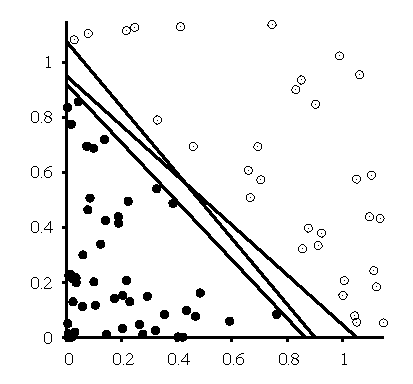
\includegraphics[width=0.4\textwidth]{resources/svm_russel_classification_a}}
%         \hspace{0.2cm}
%     \subfloat[O separador com maior margem (linha escura) no ponto médio da margem (entre as linhas tracejadas). Os vetores de suporte (pontos circulados) são os mais próximos ao separador. \label{fig:svm_classification_b}]
%         {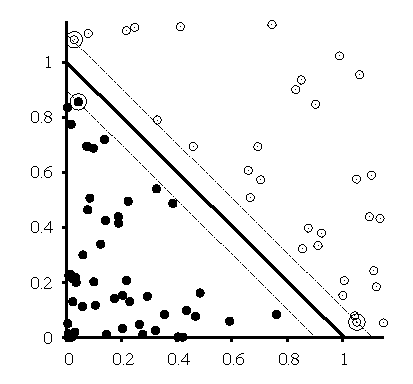
\includegraphics[width=0.4\textwidth]{resources/svm_russel_classification_b}}
%         \legend{Fonte: \citeonline[p. 745]{russell:2010}}
% \end{figure}
% %\textcolor{red}{Testes figura~\ref{fig:svm_classification}, e as figuras~\ref{fig:svm_classification_a}~e~\ref{fig:svm_classification_b}.}

% ==================================================
\subsection{Ferramentas para aprendizado de máquina}
\label{sec:ml_tools}
% ==================================================

Dada a complexidade de algoritmos de aprendizado de máquina, e visando auxiliar na produção de soluções em diversas áreas, estão disponíveis diferentes ferramentas de desenvolvimento\todo{Citar exemplos com referências}. Algumas destas ferramentas serão abordadas nas próximas seções.

% ==================================================
\subsubsection{Scikit-learn}
\label{sec:ml_sklearn}
% ==================================================

O scikit-learn é um módulo para a linguagem Python que integra uma alta gama de algoritmos\todo{Citar exemplos com referências}\ de aprendizado de máquina, tanto supervisionados quanto não supervisionados, e permite a comparação fácil de diversos métodos em uma aplicação \cite{pedregosa:2011}.

Segundo \citeonline{pedregosa:2011}, o scikit-learn aproveita o alto nível da linguagem Python para manter a facilidade de uso do \textit{framework}, tornando-o utilizável por não especialistas da indústria de software e em campos além da ciência da computação. Além disso, \citeonline{pedregosa:2011} garantem maior eficiência do que outras ferramentas semelhantes em Python, pois o scikit-learn incorpora código compilado.

\todo[inline]{Apresentar um exemplo de utilização da ferramenta, pode ser um trecho do próprio site}

% ==================================================
\subsubsection{TensorFlow}
\label{sec:ml_tf}
% ==================================================

TensorFlow é um sistema para algoritmos de aprendizado de máquina que funciona em diversos sistemas diferentes de forma flexível, sem exigir grandes alterações em uma variedade de sistemas heterogêneos \cite{abadi:2016}. É uma ferramenta bastante popular, e oferece classificação utilizando técnicas como Redes Neurais Convolutivas (CNN) e SoftMax \cite{ertram:2017}.

\todo[inline]{Ampliar esta seção está bem rasa, sugiro falar sobre as técnicas que são usadas na tool, como RNN pre-treinadas. Mencionar quem usa esta \textit{tool} e onde.}

\todo[inline]{Apresentar um exemplo de utilização da ferramenta, pode ser um trecho do próprio site}


% ==================================================
\section{Modelagem e validação de sistemas}
\label{sec:modelosformais}
% ==================================================

Sistemas embarcados são muitas vezes usados em situações críticas, em que segurança e confiabilidade são critérios muito importantes, pois podem oferecer risco à vida\todo{Apresentar exemplo}. O uso de modelos formais\todo{Citar Exemplos com referências}\ para descrever o comportamento do sistema antes que este seja desenvolvido e é uma forma de se aproximar da melhor confiabilidade, pois esses modelos podem ser validados automaticamente \cite{edwards:1997}.

% ==================================================
\subsection{Diagrama de sequência}
% ==================================================
Uma forma de detalhar as especificações iniciais do design do sistema é através do diagrama de sequência\todo{Falar um pouco sobre UML}. Este diagrama indica a troca de mensagens sequencial entre os diversos componentes de um sistema. Na figura~\ref{fig:seq_chart}, pode-se ver um exemplo de um atendedor telefônico automático. A dimensão vertical neste exemplo representa a sequência, e a horizontal representa cada componente de comunicação~\cite{marwedel:2010}.

\begin{figure}[!ht]
	\caption{\label{fig:seq_chart}Exemplo de diagrama de sequência em UML}
	\begin{center}
	    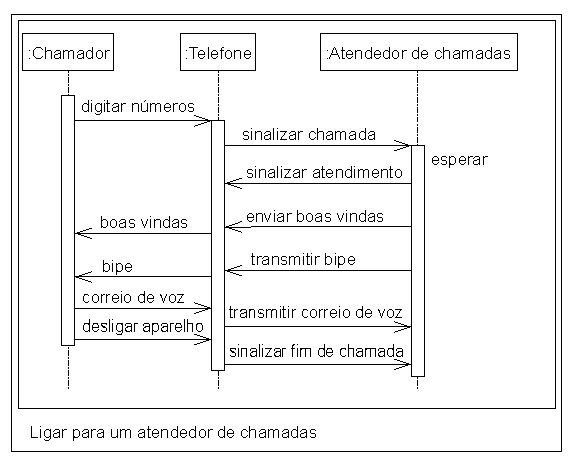
\includegraphics[width=0.8\textwidth]{resources/seq_chart_marwedel_1}
	\end{center}
	\legend{Fonte: Adaptado de \citeonline[p. 37]{marwedel:2010}}
\end{figure}

A UML contém padronização do diagrama de sequência. As linhas tracejadas representam as ``linhas da vida'', e as mensagens são ordenadas em sequência ao longo dessas linhas. Caixas sobre as linhas da vida representam controle ativo do componente correspondente. No exemplo da figura~\ref{fig:seq_chart}, as setas denotam mensagens assíncronas, e pode-se notar que a máquina espera o usuário atender o telefone. Caso isso não ocorra, a própria máquina atende e envia as boas vindas para o autor da chamada, que deixa uma mensagem no correio de voz~\cite{marwedel:2010}.

Ainda segundo \citeonline{marwedel:2010}, o diagrama de sequência tem certas limitações\todo{Exemplificar quais.} e não é capaz de descrever ações complexas, mas é útil para uma modelagem inicial.

% ==================================================
\subsection{Máquinas de Estado}
% ==================================================

A teoria dos autômatos é o estudo de dispositivos computacionais abstratos (``máquinas''), que servem de modelo para o projeto e construção de softwares, a partir de conceitos como autômatos finitos e gramáticas formais \cite{hopcroft:2001}.

Um autômato finito, também conhecido como Máquina de Estados Finita (FSM) \cite{wagner:2006}, se baseia em um conjunto finito de estados, entradas, saídas e transições entre estados. A descrição do comportamento baseado em estados é importante na modelagem de sistemas embarcados \cite{marwedel:2010}.

\todo[inline]{Apresentar definição formal para um FSM}

Cada estado de uma FSM representa uma informação sobre o decorrer do programa, pois o estado muda de tempos em tempos durante a execução, e todos os estados representam todas as situações possíveis em que a máquina de estados pode estar. As saídas podem depender tanto do estado atual quanto das entradas da máquina \cite{wagner:2006}.

\begin{figure}[ht]
	\caption{\label{fig:fsm}Exemplo de diagrama de estados}
	\begin{center}
	    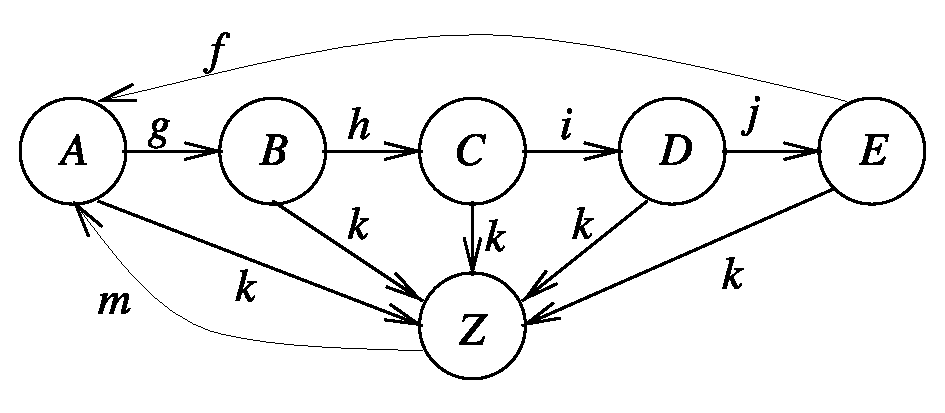
\includegraphics[width=0.6\textwidth]{resources/fsm_marwedel}
	\end{center}
	\legend{Fonte: \citeonline[p. 39]{marwedel:2010}}
\end{figure}

Um diagrama de estados como o da Figura~\ref{fig:fsm} é uma representação clássica de uma FSM. Os círculos representam estados, as arestas são transições e o rótulo das arestas são eventos de transição, que levam a máquina a mudar de estado \cite{marwedel:2010}.

A Figura~\ref{fig:fsm_2} representa um sistema de máquina de venda que aceita moedas de 5 e de 10 centavos, sendo 25 o valor esperado. O estado ``Início'' é o estado em que ainda não foi depositada uma moeda e o estado ``Fim'' quer dizer que a máquina recebeu 25 centavos. As transições representam as moedas depositadas na máquina. Em todos os estados qualquer moeda é aceita, exceto no estado ``Vinte'', em que a moeda de 10 centavos é ignorada neste exemplo por questões de simplicidade \cite{wagner:2006}.

\begin{figure}[ht]
	\caption{\label{fig:fsm_2}Diagrama de máquina de estados do contador de uma máquina de vendas}
	\begin{center}
	    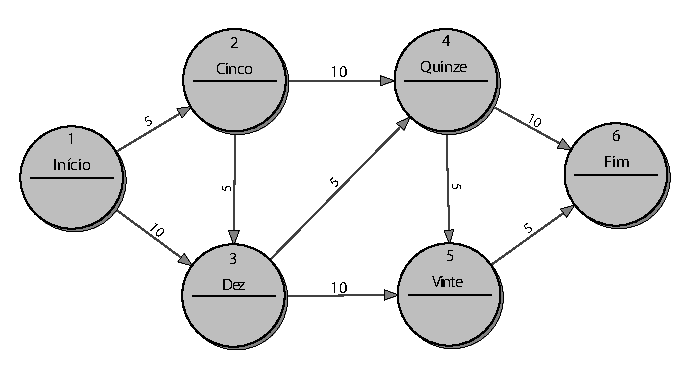
\includegraphics[width=0.8\textwidth]{resources/fsm_wagner}
	\end{center}
	\legend{Fonte: Adaptado de \citeonline[p. 68]{wagner:2006}}
\end{figure}

\todo[inline]{Descrever que propriedades podem ser validadas usando um FSM}

% ==================================================
\subsection{Redes de Petri}
% ==================================================

Uma rede de Petri é um modelo matemático de um sistema, cujo estudo pode revelar informações vitais sobre a estrutura e o comportamento do sistema modelado \cite{peterson:1981}. Segundo \citeonline{murata:1989}, as redes de Petri são uma ferramenta de modelagem matemática e gráfica, especialmente úteis para sistemas concorrentes, assíncronos, distribuídos, paralelos, não-determinísticos, e estocásticos.

A estrutura de uma rede de Petri consiste em lugares, transições, funções de entrada e funções de saída. Graficamente, sua representação é dada por um grafo direcionado, em que os lugares são representados por círculos, as transições por barras, e os arcos entre os lugares e as transições indicam entradas e saídas \cite{peterson:1981}. % $C = (P,T,I,O)

\todo[inline]{Apresentar a definição formal de RP}

Além disso, cada um dos lugares é marcado com um número não negativo de \textit{tokens}. Quando os lugares têm um número positivo $k$ de \textit{tokens}, estes são representados graficamente por $k$ círculos preenchidos posicionados no interior dos círculos que representam os lugares \cite{murata:1989}, como pode ser visto nos lugares $P_1$ e $P_2$ da figura~\ref{fig:petrinet}. Uma transição é disparada de acordo com um evento determinado, desde que hajam \textit{tokens} suficientes no lugar de entrada.

\begin{figure}[ht]
	\caption{\label{fig:petrinet}Exemplo de rede de Petri com atividades paralelas}
	\begin{center}
	    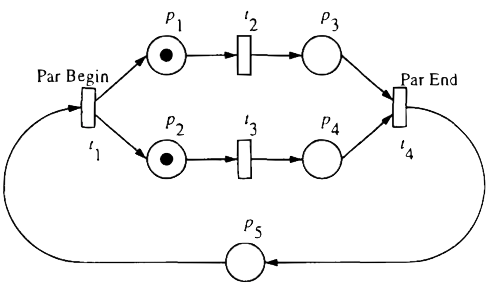
\includegraphics[width=0.5\textwidth]{resources/petri_net_murata_1}
	\end{center}
	\legend{Fonte: \citeonline[p. 545]{murata:1989}}
\end{figure}

Na \autoref{fig:petrinet} as transições $t_1$ e $t_2$ estão habilitadas, pois há \textit{tokens} suficientes nos lugares $P_1$ e $P_2$, e também são paralelas, pois suas causas são independentes. Caso uma dessas transições seja disparada, o \textit{token} no lugar de entrada é removido e um novo é produzido no lugar de saída da transição.

A partir do modelo, é possível fazer a análise da rede de Petri usando propriedades como segurança, limitação (do inglês \textit{boundedness}) e vivacidade. 
% 
Em uma rede de Petri que modela um hardware, \textit{segurança}\todo{Apresentar exemplo gráfico}\ é uma das propriedades mais importantes. Um lugar em uma rede de Petri é seguro quando nunca contém mais de um \textit{token}, e uma rede de Petri é segura se todos os lugares forem seguros. A importância desta propriedade para dispositivos de hardware se dá pelo fato de cada lugar poder ser implementado por um único \textit{flip-flop}, já que o número de um lugar pode ser apenas 0 ou 1 \cite{peterson:1981}.

O conceito de limitação\todo{Apresentar exemplo gráfico}\ é uma generalização da propriedade de segurança e determina o número \textit{k} de \textit{tokens} que são permitidos em cada lugar. Caso \textit{k} seja 1, então a propriedade de segurança se aplica. A limitação é essencial para especificação de hardware, e os lugares podem ser implementados com contadores \cite{peterson:1981}.

Um problema computacional comum em relação a alocação de recursos é o \textit{deadlock}, em que processos diferentes requerem recursos que estão indisponíveis e não conseguem prosseguir. Em uma rede de Petri, isto é representado por uma transição ou conjunto de transições que não podem ser acionadas\todo{Apresentar exemplo gráfico}. Uma transição está em \textit{deadlock} caso ela não possa ser acionada, e é uma transição \textit{viva} caso seja potencialmente acionável em qualquer situação da rede de Petri \cite{peterson:1981}.
%TODO: Considerar imagem de \textit{deadlock} de \citeonline[página 86]{peterson:1981}.

% \section{Modelagem de software}
% \label{sec:modelagem}
% \subsection{Transformações de modelo para código}

% -----------------------------------------------------------------------------
% Revisão de Literatura
% -----------------------------------------------------------------------------
\chapter{Trabalhos Correlatos}\label{ch:correlatos}
Este capítulo apresentará trabalhos existentes na literatura que compartilham de objetivos semelhantes ou são comparáveis de alguma forma e contribuem para o desenvolvimento deste trabalho. Os trabalhos descritos nas seções a seguir propõem métodos relacionados a previsão de movimentos para próteses ativas.

% ===================================================================================
\section{Translational Motion Tracking of Leg Joints for Enhanced Prediction of Walking Tasks}\label{sec:rel_stolyarov}
% ===================================================================================

Neste artigo, \citeonline{stolyarov:2017} propuseram um método de prever tarefas de caminhada utilizando apenas uma IMU (unidade de medição inercial) em uma prótese comercial de uma articulação (tornozelo-pé). Foram classificadas cinco tarefas diferentes: caminhada em solo plano, subida de rampa, descida de rampa, subida de degrau e descida de degrau.

Usando apenas a IMU, foi possível ter uma classificação até mais precisa que próteses que usam sEMG, pois, segundo os autores \citeonline{stolyarov:2017}, estas costumam ter ótimos resultados apenas em ambientes de laboratório, mas fora dele dependem de muitos fatores não controlados. A alta acurácia do classificador apresentado sugere que o método tenha ótimos resultados mesmo fora de laboratório.

Algumas limitações deste método são a falta de filtros para tratar problemas comuns do tipo de sensor utilizado, como \textit{drifting}, e a baixa precisão que o algoritmo tem em superfícies escorregadias ou macias.
% 
O estudo do artigo de \citeonline{stolyarov:2017} proporciona ao trabalho aqui proposto a noção de que o uso de acelerômetros e giroscópios pode ser o suficiente para o objetivo proposto, principalmente quando se trata de próteses de baixo custo.

% ===================================================================================
\section{Turn Intent Detection for Control of a Lower Limb Prosthesis}\label{sec:rel_pew}
% ===================================================================================

No trabalho de \citeonline{pew:2017} foi proposto fazer uma prótese para membros inferiores que tivesse rigidez adaptável em tempo real durante movimentos de virada, prevendo as ações de caminhada e de virada usando técnicas de aprendizagem de máquina, tais como, SVM e KNN\@.

A leitura dos dados foi feita a partir da simulação de uma IMU usando captura de movimentos ótica, e o controle da rigidez da articulação foi feita usando um componente chamado VSTA (\textit{variable stiffness torsion adapter}), que podia ser ativado com uma célula de carga comercialmente conhecida como iPecs, como pode ser visto na figura~\ref{fig:rel_turnintent_1}.

\begin{figure}[ht]
	\caption{\label{fig:rel_turnintent_1}Prótese incluindo o VSTA, a célula de carga iPecs e a posição da IMU simulada.}
	\begin{center}
	    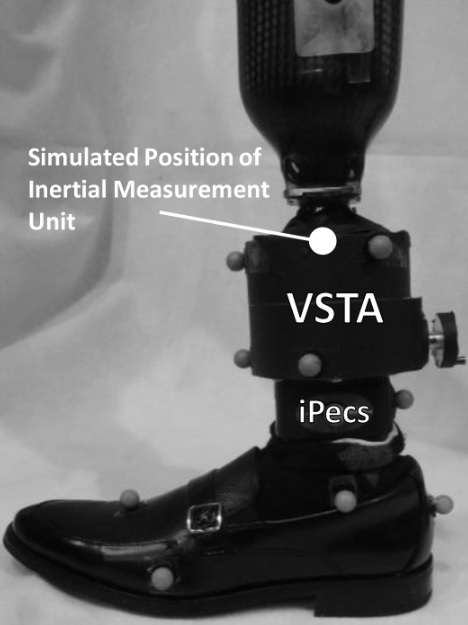
\includegraphics[width=.25\textwidth]{resources/rel_pew_turnintent_1}
	\end{center}
	\legend{Fonte: \citeonline{pew:2017}}
\end{figure}

Para a previsão de ações, foi feita uma comparação entre técnicas de classificação em aprendizagem de máquina: \textit{Bagged Decision Tree Ensemble}~\cite{breiman:1996bagging}\cite{dietterich:2000ensemble}, SVM~\cite{cortes:1995svm} e KNN~\cite{cover:1967knn}\@. Na previsão de caminhada, o SVM teve $85\%$ de acurácia, o KNN teve $82\%$, e o \textit{Ensemble}, $97\%$. Na previsão de virada, o SVM teve $96\%$, o KNN, $93\%$ e o \textit{Ensemble} teve $91\%$ de acurácia.

Embora tenha sido inferior na classificação da intenção de virada, a alta acurácia do \textit{Bagged Decision Tree Ensemble} na detecção de caminhada compensa, o que o torna o algoritmo mais preciso dentre os testados. Também foi constatado, através da IMU simulada, que a acurácia do giroscópio ($83\%$ a $90\%$) foi superior à do acelerômetro ($66\%$ a $77\%$), o que conclui que o uso apenas do giroscópio pode ser suficiente.

A comparação dos algoritmos feita pelos autores \citeonline{pew:2017} e os testes feitos com a IMU simulada podem ser úteis para este trabalho, pois valida a utilização dos sensores como forma de leitura de movimentos para previsão de intenções.


% ===================================================================================
\section{Automated detection of gait initiation and termination using wearable sensors}\label{sec:rel_novak}
% ===================================================================================

\citeonline{novak:2013Automated} desenvolveram um método de previsão de início e término de caminhada, a partir de IMUs e uma sola sensível a pressão. O treino foi feito com pessoas com membros intactos e sem deficiências motoras, apenas para desenvolver a técnica. Foram utilizados \(12\) sinais das IMUs, passando por filtros de Kalman~\cite{kalman:1960}, e \(4\) sinais das duas solas. Além disso, os sinais foram classificados utilizando uma árvore de classificação, tanto para detectar os passos individuais quanto para prever as intenções de início e término da caminhada.

No trabalho de \citeonline{novak:2013Automated} foi constatado que é possível detectar o início da caminhada usando a velocidade angular do quadril e ângulo do joelho; e o término utilizando a duração dos passos, e o padrão da pisada na sola para detectar se o passo atual será o último.

Ainda segundo \citeonline{novak:2013Automated}, IMUs são mais eficientes para detectar o término da caminhada, e os sensores nas solas são melhores para detectar os passos individuais. O sistema pode ser adaptado para ser usado em dispositivos como próteses ou exoesqueletos, embora precise ser reduzido para isso, devido à grande quantidade de sensores.

% A técnica apresentada pareceu ser eficiente, porém a grande quantidade de sensores não a torna muito prática fora de um laboratório.

% ===================================================================================
\section{A Novel Design of a Full Length Prosthetic Robotic Arm for the Disabled}\label{sec:rel_kumar}
% ===================================================================================

% \todo[inline]{\textbf{ATENÇÃO:} Achei esse artigo muito ``engenharia'', pois não fala sobre a classificação em si, e foca muito na construção do braço, incluindo a escolha de materiais.}

O trabalho de \citeonline{kumar:2017} propõe um protótipo de braço prostético robótico (ver Figura~\ref{fig:rel_kumar_1}) controlado por um microcontrolador, com uso de aprendizagem de máquina. Além disso, o objetivo era fazer com que a prótese tivesse movimentos com aspecto humano e o menor torque necessário possível.

\begin{figure}[!htp]
	\caption{\label{fig:rel_kumar_1}Modelagem do protótipo desenvolvida no Solid Works}
	\begin{center}
	    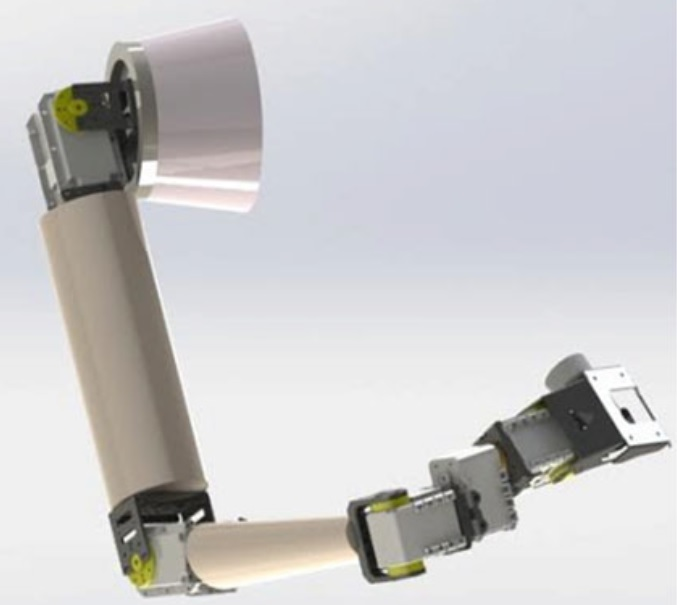
\includegraphics[width=.3\textwidth]{resources/rel_kumar_1}
	\end{center}
	\legend{Fonte: \citeonline{kumar:2017}}
\end{figure}

O protótipo de \citeonline{kumar:2017} foi desenvolvido usando o \textit{software} Solid Works\footnote{<https://www.solidworks.com/>}, e a simulação foi feita com Simulink\footnote{<https://www.mathworks.com/products/simulink.html>} e SimMechanics\footnote{<https://www.mathworks.com/products/simmechanics.html>}. A classificação por aprendizado de máquina foi feita utilizando ANFIS~\cite{jang:1993anfis}, um tipo de rede neural artificial, a partir dos dados gerados na simulação.

Foram geradas 40 mil posições do braço, simulando um braço humano real. Estes dados foram utilizados para treinar o algoritmo ANFIS, que então foi capaz de determinar o ângulo das articulações. Para atuar nos movimentos do braço robótico, foram usados vários servomotores e um microcontrolador PIC16F886.


% ===================================================================================
\section{SmartLeg: An intelligent active robotic prosthesis for lower-limb amputees}\label{sec:rel_smartleg}
% ===================================================================================

O trabalho de \citeonline{dedic:2011} propõe uma forma de transformar uma prótese passiva disponível comercialmente em ativa, para que seja possível a subida e descida de escadas e outros movimentos que exigem um maior esforço motor. Assim, fez-se necessário o uso de uma fonte de energia externa, que foi feita usando atuadores hidráulicos nas articulações, como visto na Figura~\ref{fig:rel_smartleg_1}.

\citeonline{dedic:2011} também discute o uso de aprendizagem de máquina para garantir conforto aos usuários, pois pode-se adaptar os atuadores para funcionarem melhor com os padrões de andadura do indivíduo, mas isso não foi implementado. Outra ideia mencionada foi o uso de sensores de proximidade e sonares para detecção de obstáculos, algo que também não foi testado, apenas sugerido para o futuro.

\begin{figure}[ht]
	\caption{\label{fig:rel_smartleg_1}Protótipo com dois atuadores hidráulicos: nas articulações do joelho e do tornozelo.}
	\begin{center}
	    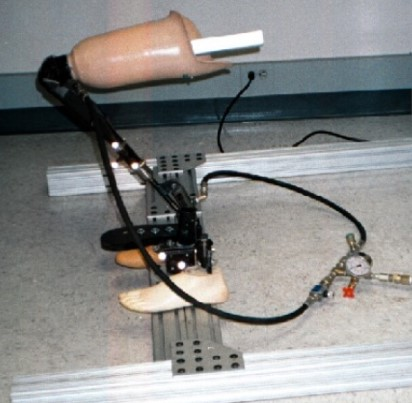
\includegraphics[width=.35\textwidth]{resources/rel_dedic_smart_leg_1}
	\end{center}
	\legend{Fonte: \citeonline{dedic:2011}}
\end{figure}

O protótipo da Figura~\ref{fig:rel_smartleg_1} foi desenvolvido visando baixo custo, pois utiliza uma prótese passiva disponível no mercado, apenas a equipando com atuadores. A coleta de dados realizada permitiu que se comparasse o padrão de caminhada de indivíduos saudáveis com amputados utilizando a prótese, e a prótese produzida permitiu dois graus de liberdade (DOF) com o controle feito por microcontrolador. O maior empecilho é o sistema hidráulico utilizado, que ocupa muito espaço, tornando a versão proposta atual inviável para uso diário.

%\section{Evaluation of shoulder complex motion-based input strategies for endpoint prosthetic-limb control using dual-task paradigm}
%\todo[inline]{\cite{losier:2011}}

%\section{Movement error rate for evaluation of machine learning methods for sEMG-based hand movement classification}
%\todo[inline]{\cite{gijsberts:2014}}



% -----------------------------------------------------------------------------
% Detalhes de Desenvolvimento do Projeto
% -----------------------------------------------------------------------------
\chapter{Método Proposto}\label{ch:metodo}
Este capítulo apresentará o método proposto por este trabalho para o projeto de prótese ativa baseada em sensores e aprendizado de máquina.

\section{\todo{Corrigir este título}A prótese}
\label{sec:metodo_protese}
\todo[inline]{Explicar o funcionamento geral, relacionando à big picture}
\label{sec:metodo_geral}
\begin{figure}[h]
	\caption{\label{fig:big_picture}Visão geral do protótipo}
	\begin{center}
	    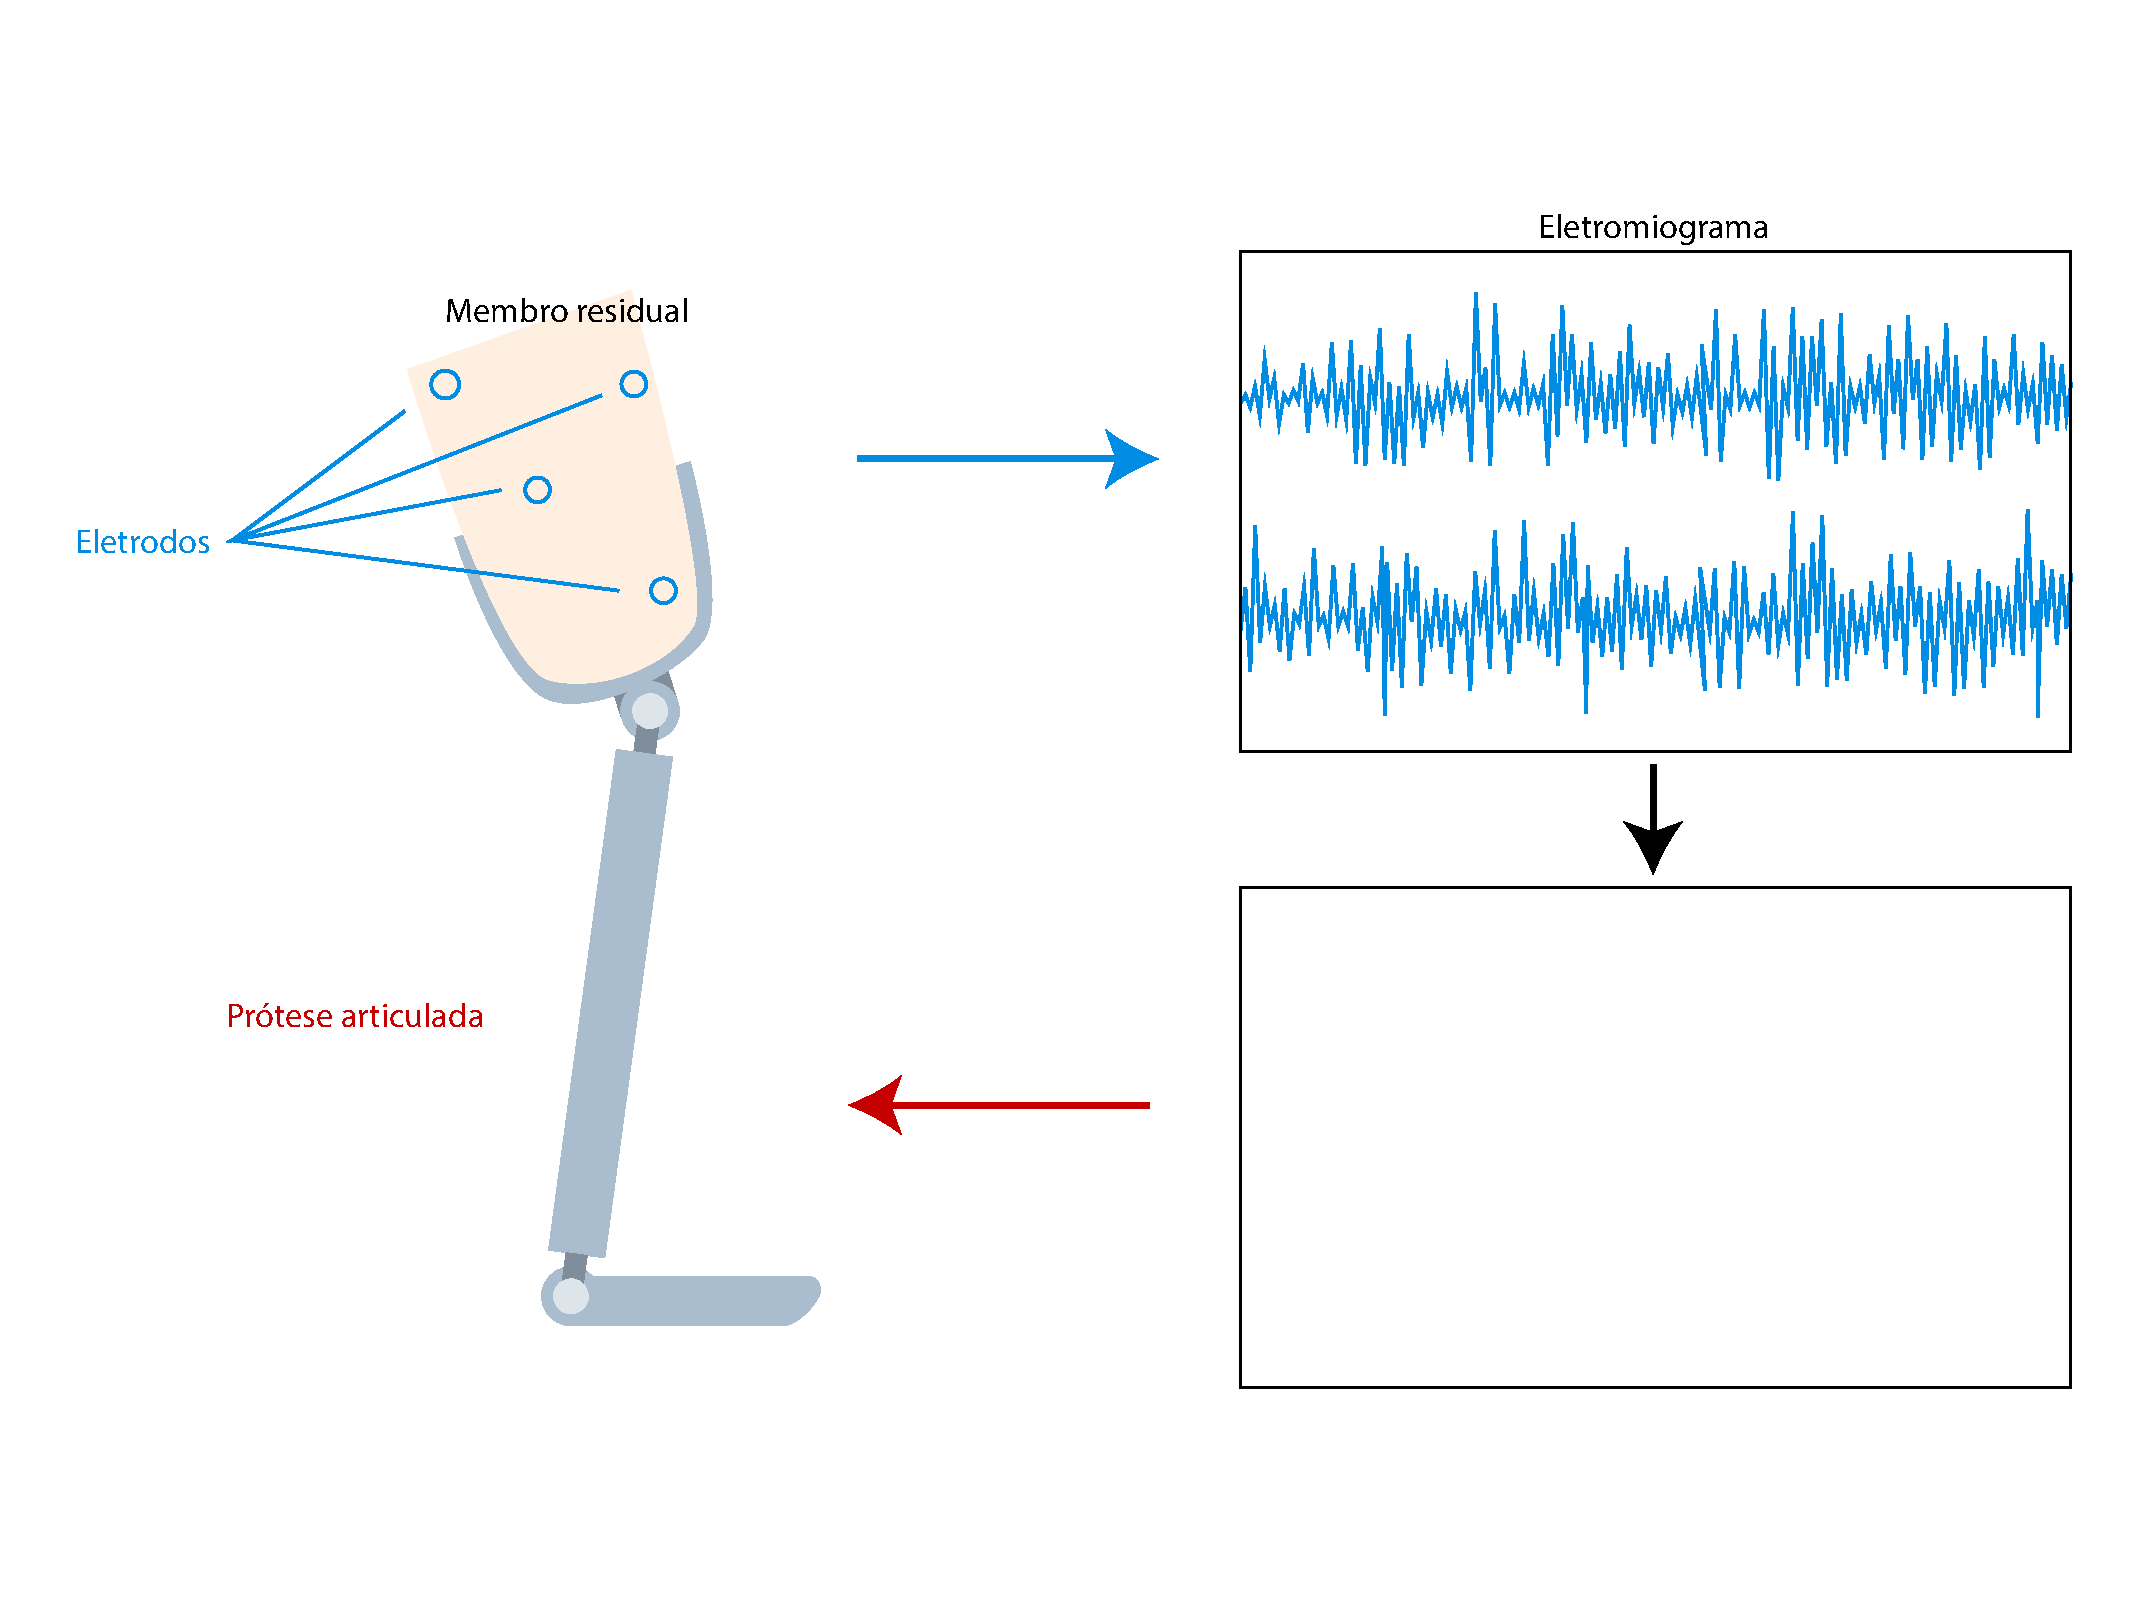
\includegraphics[width=0.8\textwidth]{resources/big_picture}
	\end{center}
	\legend{Fonte: Elaborada pelo autor}
\end{figure}

\todo[inline,color=lightgray]{Projeto e prototipação de uma prótese robótica para pé\\Como criar;\\Onde vão estar os sensores, materiais de baixo custo, próteses 3D;\\O que a prótese gera?; Atuadores; Gerar perguntas.}
\todo[inline]{Como vai ser a fonte de energia da prótese?}

\section{Coleta de dados e classificação}
\todo[inline,color=lightgray]{Coleta de dados dos sensores -- que sensores, que dados. Por que os dados são importantes: usar técnicas pra prever e identificar dados (Seção explicando da coleta, uma seção pra cada tipo de classificação)}

\todo[inline]{\textbf{Nova seção?}}
\todo[inline,color=lightgray]{Geração de movimentos: a partir dos dados coletados. Os atuadores vão tentar identificar os ambientes. Na escada, o motor vai fazer tal coisa, etc. Na rampa, etc.}

\todo[inline]{\textbf{Nova seção?}}
\todo[inline,color=lightgray]{Analisar saúde do caminhar. Se não tá caminhando torto. Gerar estatísticas do uso da prótese. (Os dados estão fazendo a pessoa puxar mais pra uma perna)}

% -----------------------------------------------------------------------------
% Cronograma
% -----------------------------------------------------------------------------
\chapter{Cronograma}\label{ch:cronograma}
\todo[inline]{Fazer cronograma}
\begin{table}[htbp]
  \centering
  \caption{Cronograma de atividades}
  \label{tab:cronograma}
  \begin{tabular}{|c|c|c|c|c|c|}
    \hline
    \textbf{Atividade} & \textbf{Março} & \textbf{Abril} & \textbf{Maio} & \textbf{Junho} & \textbf{Julho} \\
    \hline
    Elaboração do projeto & \(\times\) & & & & \\
    \hline
    Revisão da literatura & & \(\times\) & & & \\
    \hline
    Metodologia & & & \(\times\) & & \\
    \hline
    Conceitos e Definições & & & & \(\times\) & \\
    \hline
    Entrega do trabalho para banca & & & & & \(\times\) \\
    \hline
    Defesa para a banca & & & & & \(\times\) \\
    \hline
  \end{tabular}
  %\legend{Fonte: Autor.}
\end{table}
%\newpage
% -----------------------------------------------------------------------------
% Referências bibliográficas
% -----------------------------------------------------------------------------
%\bibliographystyle{abnt-alf}
\bibliography{main}

% -----------------------------------------------------------------------------
% ÍNDICE REMISSIVO
% -----------------------------------------------------------------------------
%\phantompart
\printindex
% -----------------------------------------------------------------------------

\end{document}
